%% 
%% Copyright 2007-2020 Elsevier Ltd
%% 
%% This file is part of the 'Elsarticle Bundle'.
%% ---------------------------------------------
%% 
%% It may be distributed under the conditions of the LaTeX Project Public
%% License, either version 1.2 of this license or (at your option) any
%% later version.  The latest version of this license is in
%%    http://www.latex-project.org/lppl.txt
%% and version 1.2 or later is part of all distributions of LaTeX
%% version 1999/12/01 or later.
%% 
%% The list of all files belonging to the 'Elsarticle Bundle' is
%% given in the file `manifest.txt'.
%% 
%% Template article for Elsevier's document class `elsarticle'
%% with harvard style bibliographic references

%\documentclass[preprint,12pt,authoryear]{elsarticle}

%% Use the option review to obtain double line spacing
%% \documentclass[authoryear,preprint,review,12pt]{elsarticle}

%% Use the options 1p,twocolumn; 3p; 3p,twocolumn; 5p; or 5p,twocolumn
%% for a journal layout:
%% \documentclass[final,1p,times,authoryear]{elsarticle}
%% \documentclass[final,1p,times,twocolumn,authoryear]{elsarticle}
%% \documentclass[final,3p,times,authoryear]{elsarticle}
%% \documentclass[final,3p,times,twocolumn,authoryear]{elsarticle}
%% \documentclass[final,5p,times,authoryear]{elsarticle}
 \documentclass[final,5p,times,twocolumn,authoryear]{elsarticle}

%% For including figures, graphicx.sty has been loaded in
%% elsarticle.cls. If you prefer to use the old commands
%% please give \usepackage{epsfig}

%% The amssymb package provides various useful mathematical symbols
\usepackage{amssymb}
\usepackage{lipsum}
\usepackage{amsmath}
\usepackage{geometry}
\usepackage{float}%% The amsthm package provides extended theorem environments
%% \usepackage{amsthm}
\usepackage{placeins}
\usepackage{booktabs}
\usepackage{microtype}
\usepackage{comment}
\usepackage{pgfplots}
\usepackage{url}
\usepackage[hidelinks]{hyperref}
\def\UrlBreaks{\do\/\do-\do\_\do\.\do\?\do\&}
%% The lineno packages adds line numbers. Start line numbering with
%% \begin{linenumbers}, end it with \end{linenumbers}. Or switch it on
%% for the whole article with \linenumbers.
%% \usepackage{lineno}

%% You might want to define your own abbreviated commands for common used terms, e.g.:
\newcommand{\kms}{km\,s$^{-1}$}
\newcommand{\msun}{$M_\odot$}

\journal{Results in Physics}


\begin{document}

\begin{frontmatter}

%% Title, authors and addresses

%% use the tnoteref command within \title for footnotes;
%% use the tnotetext command for theassociated footnote;
%% use the fnref command within \author or \affiliation for footnotes;
%% use the fntext command for theassociated footnote;
%% use the corref command within \author for corresponding author footnotes;
%% use the cortext command for theassociated footnote;
%% use the ead command for the email address,
%% and the form \ead[url] for the home page:
%% \title{Title\tnoteref{label1}}
%% \tnotetext[label1]{}
%% \author{Name\corref{cor1}\fnref{label2}}
%% \ead{email address}
%% \ead[url]{home page}
%% \fntext[label2]{}
%% \cortext[cor1]{}
%% \affiliation{organization={},
%%            addressline={}, 
%%            city={},
%%            postcode={}, 
%%            state={},
%%            country={}}
%% \fntext[label3]{}

\title{Leakage Detection in Water-Distribution-Networks using Physics-Aware Artificial Neural Networks and Leakage Localization using a Rule-based System}

%% use optional labels to link authors explicitly to addresses:
%% \author[label1,label2]{}
%% \affiliation[label1]{organization={},
%%             addressline={},
%%             city={},
%%             postcode={},
%%             state={},
%%             country={}}
%%
%% \affiliation[label2]{organization={},
%%             addressline={},
%%             city={},
%%             postcode={},
%%             state={},
%%             country={}}


% Authors (all equal contribution)
\author[inst1,eq]{Jash Shah}
\author[inst1,eq]{David Daniels}
\author[inst1,eq]{Heet Shah}
\author[inst1,eq]{Abhijeet Salunke}

\vspace{0.3cm}

% Affiliation
\affiliation[inst1]{
  organization={Department of Computer Engineering, Sardar Patel Institute of Technology},
  addressline={Mumbai},
  country={India}
}

% Footnotes
\fntext[eq]{All authors contributed equally to this work.}
\fntext[]{\{jash.shah23, david.daniels23, heet.shah223, abhijeet\_salunke\}.spit.ac.in}

\begin{abstract}
%% Text of abstract
We present a Physics-Aware Artificial Neural Network (PAANN) for leak detection in Water Distribution Networks (WDNs). Unlike purely data-driven approaches, our model embeds conservation of mass and energy (via the continuity equation and Hazen-Williams relation) into the training loss, ensuring physically consistent predictions. We compare the Physics-Aware ANN against a base ANN and XGBoost on the LeakDB Hanoi dataset. The Physics-Aware ANN achieves superior F1 (0.8598) and precision (0.9659), with a 62.98\% reduction in false positives compared to the base ANN, while maintaining strong recall. Leak localization is performed via a rule-based post-processing step. Our results demonstrate that incorporating hydraulic physics into neural network training improves detection reliability and reduces false alarms.
\end{abstract}

%%Graphical abstract
\begin{graphicalabstract}
\includegraphics{grabs}
\end{graphicalabstract}

%%Research highlights
\begin{highlights}
\item Research highlight 1
\item Research highlight 2
\end{highlights}

\begin{keyword}
%% keywords here, in the form: keyword \sep keyword, up to a maximum of 6 keywords
Water distribution networks \sep Leak detection \sep Physics-aware neural networks \sep Conservation of mass \sep Hazen-Williams \sep LeakDB

%% PACS codes here, in the form: \PACS code \sep code

%% MSC codes here, in the form: \MSC code \sep code
%% or \MSC[2008] code \sep code (2000 is the default)

\end{keyword}


\end{frontmatter}

%\tableofcontents

%% \linenumbers

%% main text

\section{Introduction}
\label{introduction}

\subsection{Motivation and Relevance}
Water is one of the most essential resources for human survival, economic growth, and sustainable urban development. With rapid urbanization and increasing population density in major towns and cities, Water Distribution Networks (WDNs) have become more extensive and complex.  These networks are responsible for delivering potable water from natural water bodies or reservoirs to consumers, and their efficient operation is crucial to ensure water security and sustainability.
The volume of leakages in WDNs varies throughout different geographies, and the primary factors affecting the amount of water lost due to leakage are the general condition of the network and the maintenance and monitoring system in place. Some places suffer from as much as 70-80\% loss in water due to leakages, while where the infrastructure is secure, the lost water volume is around 7-8\%. In total, worldwide, the amount of non-revenue water (NRW) is around 126 billion cubic meters annually, and corresponding to a monetary loss of approximately 39 billion USD annually

\subsection{Challenges}
Monitoring systems for WDNs are primarily acoustic monitoring systems, or they rely heavily on manual inspection and are labor-intensive, time-consuming, and costly. Recent advancements in data-driven methods and sensor-based monitoring have improved detection accuracy; however, many of these approaches rely heavily on data-driven and complex models that do not explicitly incorporate the underlying physical laws of fluid dynamics. As a result, their predictions may lack physical interpretability and generalization in unseen scenarios.

\subsection{Contribution}
Our Physics-Aware ANN (PAANN) integrates physical laws into the model latent space so that predictions do not violate the equations and laws of conservation of mass and energy. The model vastly reduces the number of false positives, saving both monetary and human cost by predicting a leak only when the model is highly confident. This is a comparatively low-cost solution that can be generalized for any WDN, and our localization method predicts the leakage area using a relatively simple set of rules, not relying on expensive models for localization that are both time- and compute-intensive.

\section{Related work}

The detection and localization of leaks in Water Distribution Networks (WDNs) have been
 investigated through various methods. This section presents a synthesis of recent advances, organized into subsections covering methodologies ranging from traditional data-driven machine learning approaches to physics-informed ones, along with the research gap motivating the present study.

\subsection{Traditional Data-Driven Approaches}

Classical machine learning and deep learning methods have demonstrated considerable promise in leak detection, primarily by learning patterns from historical operational data. \cite{MAHDI2024100685} employed advanced statistical features—specifically, Autocorrelation Coefficient (Au-C) and Signal Energy (Sig-E)—extracted from accelerometer and dynamic pressure sensor measurements. Their Artificial Neural Network (ANN) achieved accuracies of 86.5\% and 86.2\% F1-scores for branched and looped configurations, respectively. The study highlighted the efficacy of data fusion in enhancing detection reliability; however, the approach remained purely empirical, lacking integration with underlying hydraulic principles.

Similarly, \cite{sousa2023leakagedetection} investigated machine learning strategies including K-means clustering, Learning Vector Quantization (LVQ), and cluster validation techniques on data from a District Metered Area (DMA) in Stockholm, Sweden. Their methodology achieved classification rates up to 93.98\%, demonstrating robustness to common sensor noise levels within ±5\%. Nonetheless, the authors acknowledged limitations in handling dynamic operational variations and the absence of physical interpretability in model predictions.

Deep learning architectures have also been explored. \cite{punukollu2023leakdetection} applied Convolutional Neural Networks (CNN) and Long Short-Term Memory (LSTM) networks on the LeakDB benchmark dataset \cite{kyriakou2018leakdb}, achieving leak detection accuracies ranging from 49\% to 98.23\% depending on network complexity. While these models captured temporal dependencies effectively, they required extensive labeled training data and exhibited reduced generalization under distribution shifts—a common challenge in purely data-driven paradigms.

\subsection{Hybrid and Model-Based Methodologies}

Recognizing the limitations of purely data-driven approaches, recent research has integrated hydraulic modeling with statistical or machine learning techniques. \cite{mazaev2022probabilisticleaklocalization} proposed a hybrid framework combining EPANET hydraulic simulations with a Time-Windowed Head Bias Correction (TWHBC) mechanism and an Elastic-Net logistic regression classifier. Their approach explicitly accounted for model-data discrepancies through bias correction and achieved leak localization within predefined search radii for multiple in-field experiments. However, the methodology's reliance on accurate hydraulic model calibration and computational overhead limited its real-time applicability.

\cite{barros_leak_2025} introduced a multilayer network representation integrating topological, correlation-based, and sensor coverage graphs. By combining graph theory with statistical anomaly detection (z-score and Interquartile Range), they successfully detected leaks within 15 minutes and localized them within a 50-meter range in the BattLeDIM benchmark network. Their approach reduced the need for exhaustive hydraulic simulations by regionalizing search spaces; nevertheless, the framework struggled with incipient leaks exhibiting gradual flow increases, underscoring the necessity for continuous physical constraint enforcement.

\subsection{Physics-Informed Neural Networks in WDNs}

Physics-Informed Neural Networks (PINNs) represent an emerging paradigm that embeds governing partial differential equations (PDEs) directly into neural network loss functions, ensuring adherence to known physical laws. \cite{TORNYEVIADZI2023106062} pioneered the application of a 1D CNN deep autoencoder with semi-supervised learning on multivariate SCADA data from the L-TOWN benchmark network. Their PINN-based framework incorporated continuity and momentum equations via Pruned Exact Linear Time (PELT) change point detection, achieving identification of 16 out of 19 leaks and accurate localization of 13 within a 300-meter radius—without requiring a calibrated hydraulic model. The study demonstrated minimal identification lag for abrupt leaks, though incipient leaks remained challenging.

Expanding on this foundation, \cite{falas2020pinnwatersecurity} explored PINNs for cybersecurity applications in WDNs, specifically mitigating sensor-based cyberattacks. By training surrogate models on Navier-Stokes equations, they achieved predictive accuracies exceeding 99\% for velocity fields, enabling the detection of data integrity attacks within simulated environments. While conceptually innovative, the work focused on small-scale proof-of-concept scenarios and did not address scalability to operational networks.

More recently, \cite{lin2025digitaltwin} developed a digital twin framework leveraging PINNs for pipeline leakage detection in Taiwan's water infrastructure. Their model embedded continuity and momentum equations into the loss function and utilized statistical control charts (z-score and IQR) on reconstruction errors to detect anomalies. Validation on real-world datasets yielded R² values of 88.91\% and 98.91\% for small- and large-scale networks, respectively, with leak detection within 15 minutes of occurrence. Despite these successes, the framework's dependency on accurate boundary conditions and its limited handling of transient flow regimes were noted as areas requiring further investigation.

\subsection{Leak-Specific Physics-Informed Approaches}

Recent studies have moved beyond generic physics-informed modeling toward frameworks explicitly tailored for leak detection and localization in Water Distribution Networks (WDNs), integrating learning with hydraulic constraints to better capture leak-induced anomalies.

\cite{ORNGARDARSSON2022661} proposed a physics-informed graph neural network framework that embeds mass conservation and pressure–flow relationships directly into the learning process for leak localization. By representing the WDN as a graph and propagating leak-induced pressure residuals across adjacent nodes, the model exploited spatial correlations inherent in the network topology to improve localization accuracy. The incorporation of physics-based loss terms significantly reduced false positives compared to purely data-driven GNN baselines, particularly under moderate sensor noise conditions. Experimental validation demonstrated improved robustness to measurement uncertainty and partial observability. However, the approach primarily operated under quasi-steady-state assumptions and exhibited limited sensitivity to gradual or incipient leaks, where pressure deviations evolve slowly over time.

This work represents closely aligned prior research, demonstrating that leak-specific physics-informed learning can substantially enhance detection reliability and interpretability. Nevertheless, such graph-based frameworks predominantly emphasize spatial correlations and require graph-structured inputs. The integration of mass and energy conservation constraints within dense feed-forward architectures—which can operate on flattened sensor data without explicit graph construction—remains underexplored for leak detection, motivating our Physics-Aware ANN approach.

\subsection{Benchmark Datasets and Evaluation Challenges}

The availability of standardized datasets is crucial for reproducible research. \cite{kyriakou2018leakdb} introduced LeakDB, a publicly available benchmark comprising EPANET-simulated scenarios for multiple WDN topologies (including Hanoi, Net1) with annotated leak events. The dataset facilitates comparative evaluation but has been critiqued for relying solely on simulated data, potentially limiting model robustness under real-world operational uncertainties.

Comparative studies on BattLeDIM \cite{barros_leak_2025} and other benchmarks reveal persistent challenges: high false positive rates for incipient leaks, computational overhead in large-scale networks, and difficulty in achieving physically interpretable predictions under domain shifts. These gaps motivate the integration of physics-informed constraints within scalable neural network architectures.

\subsection{Research Gaps and Motivation}

Despite substantial progress, existing methodologies exhibit critical limitations:

\begin{itemize}
    \item \textbf{Lack of Physical Interpretability:} Purely data-driven models \cite{MAHDI2024100685, punukollu2023leakdetection} achieve high accuracies but fail to guarantee adherence to conservation laws, limiting generalization and trustworthiness.
    \item \textbf{Computational Scalability:} Hybrid approaches \cite{mazaev2022probabilisticleaklocalization} and traditional PINNs \cite{lin2025digitaltwin} often require extensive hydraulic simulations or suffer from high computational costs in large networks.
    \item \textbf{Incipient Leak Detection:} Methods leveraging statistical anomaly detection \cite{barros_leak_2025, TORNYEVIADZI2023106062} struggle with gradual leak growth due to subtle signal variations.
    \item \textbf{Integration of Physics with Dense Architectures:} While graph-based and PINN approaches have been explored, the integration of mass and energy conservation constraints within dense feed-forward architectures for leak detection remains underexplored.
\end{itemize}

Addressing these gaps, the present study proposes a \textbf{Physics-Aware Artificial Neural Network (PAANN)} framework that embeds conservation of mass and the Hazen-Williams relation directly into a fully connected feed-forward architecture. By using the LeakDB Hanoi dataset, we aim to achieve physically consistent and computationally efficient leak detection and localization, advancing beyond existing data-driven and hybrid methodologies.

\section{What is a Physics-Aware Neural Network?}

\subsection{Physics-Informed Neural Networks (PINNs)}
PINNs are neural networks that solve \textbf{\textit{continuous partial differential equations (PDEs)}} that govern physical systems. This is done by embedding differential equations into the model training. The derivatives are calculated using \textbf{\textit{automatic differentiation.}} The loss is defined as the PDE residual, evaluated at points in the continuous domain.

\subsection{Physics-Aware Neural Networks (PANNs)}
In comparison, as our data are discrete (at 30-minute time-steps), we use PANNs. Here the model predicts the physical quantities alongside its primary goal, and the predicted values are used to compute the residuals of mass and energy conservation using formulae appropriate for the data. The normalized residuals are added to the data loss for backpropagation, and the predicted values also feed into the classification head. \textbf{Compared to PINNs, PANNs require significantly less training time and compute while yielding improved performance over baseline models.}

\begin{figure}[H]
    \centering
    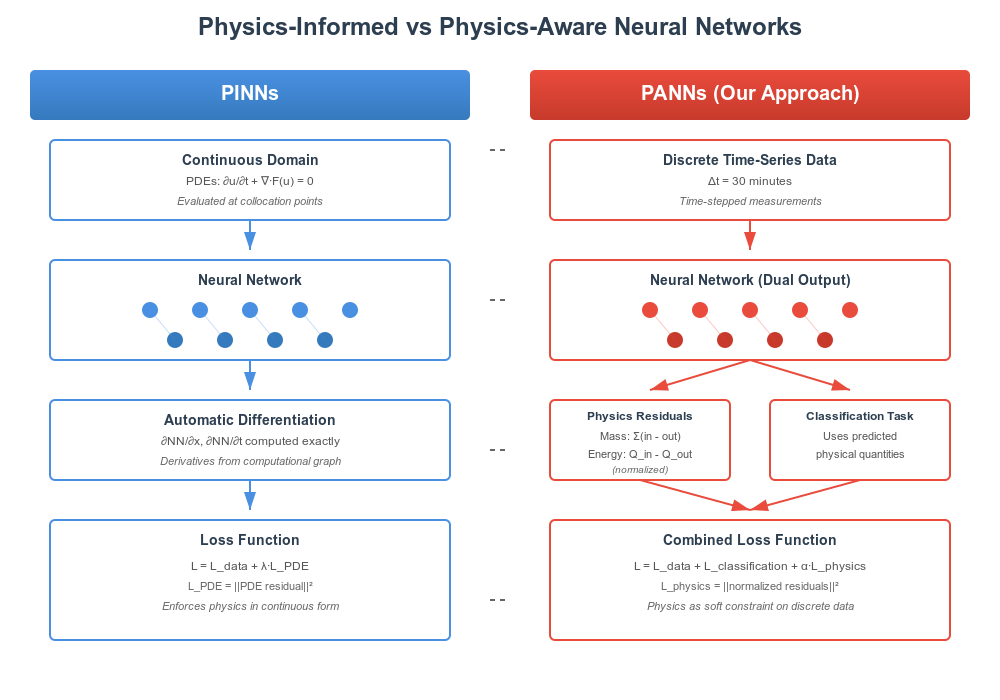
\includegraphics[width=1.1\linewidth]{pinn_pann_comparison.png}
    \caption{PINN vs PANN}
    \label{fig:diagram}
\end{figure}

\subsection{Localization methods}

\subsection{Research Gap}

\section{Problem Formulation and System Overview}

\subsection{Problem Definition}

\subsection{Mathematical Formulation}

\subsection{System Overview Diagram}

\section{Dataset}

\subsection{Dataset Description}

This study uses the LeakDB Hanoi dataset, which is made using the \textit{Water Network Resilience Tool (WNTR)}. The dataset consists of a total of 999 scenarios, where each scenario is a different simulation of the Hanoi WDN for a year. The data points in each scenario are thirty minutes apart, which means there are 17,520 data points in one scenario, and a total of 17,502,480 data points in the entire dataset. 

The Hanoi WDN consists of 32 nodes and 34 pipes connecting them, and the LeakDB dataset assumes pressure, demand and flow-rate sensors at these 32 nodes. Thus, each data point has 32 demand readings, 32 pressure readings, and 34 flow-rate readings, making a total of 98 values per time-step.

\begin{figure}[H]
    \centering
    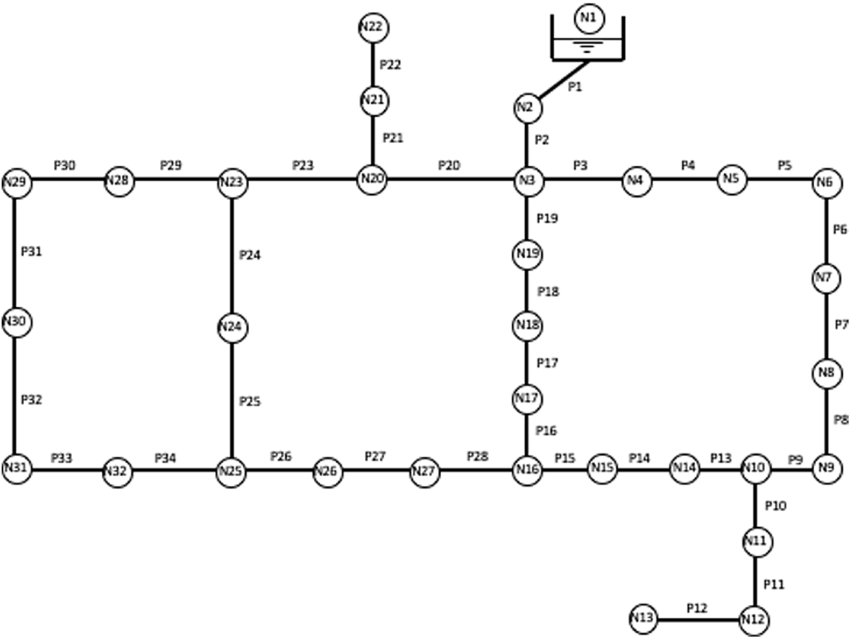
\includegraphics[width=\linewidth]{hanoi-wdn.png}
    \caption{Figure of Hanoi WDN}
    \label{fig:diagram}
\end{figure}

The data can be downloaded using the \texttt{water\_benchmark\_hub} Python module. There are two types of reading available, namely \textit{raw\_data} and \textit{scada\_data}. In this work, \textit{raw\_data} is used, as it also includes readings of demand.

Initially, each scenario is stored as a directory containing subfolders for \textit{demand}, \textit{pressure}, \textit{flow}, and \textit{leaks}, where leak labels are multi-class values ranging from 0 to 32. In addition, each scenario includes an \textit{INP} file, which specifies the simulated length, diameter, and roughness coefficient of each pipe. For the learning task, the dataset is reformatted into a single \texttt{.csv} file per scenario, where leak labels are converted to a binary representation (leak / non-leak). 

Leak localization is not learned directly by the model and is instead performed as a post-processing step using a rule-based system.


\subsection{Exploratory Analysis of Data}

Below is the heatmap of all 999 scenarios with 5\% rows from each scenario selected randomly. The demand and pressure readings show a consistent negative correlation, reflecting a drop in pressure when demand increases or vice-versa. Flow readings show mixed correlations with demand and pressure, indicating the directional and topological effects of the network. These correlations support the use of dense models and also physics-aware models.

\begin{figure}[H]
    \centering
    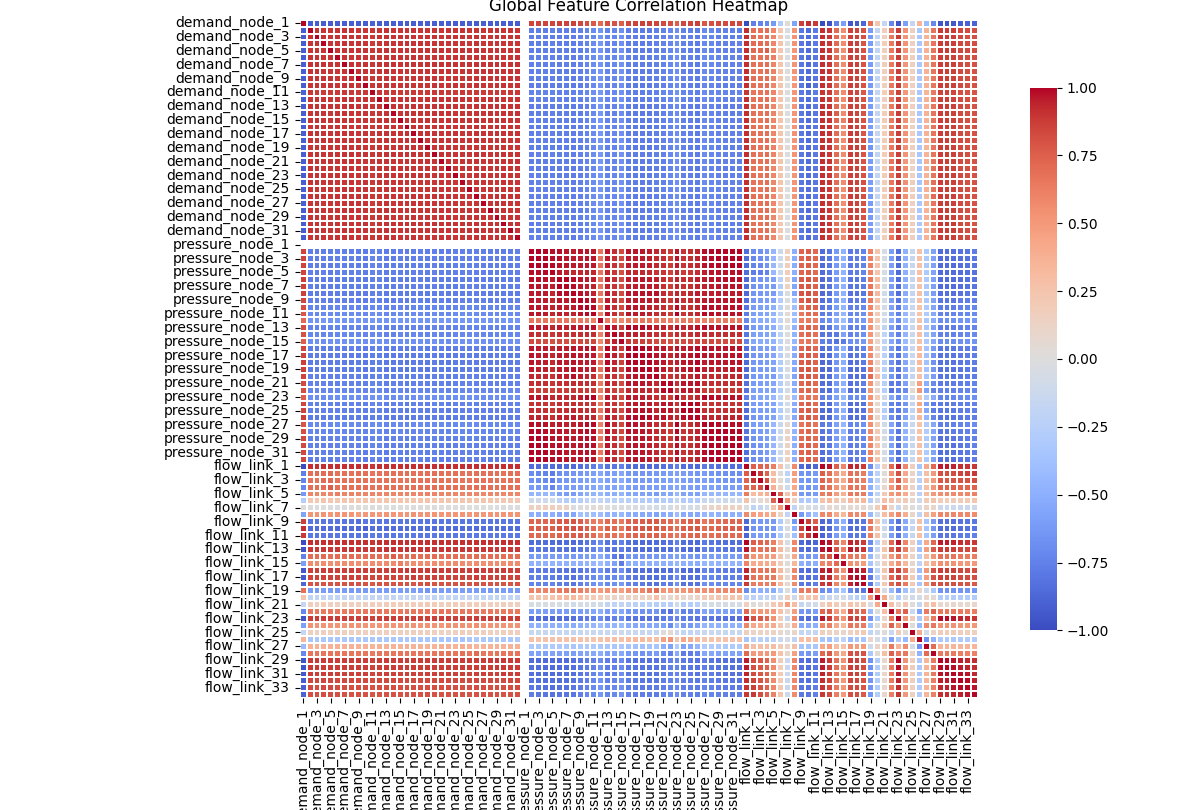
\includegraphics[width=\linewidth]{heatmap.png}
    \caption{Correlation heatmap of Hanoi WDN}
    \label{fig:diagram}
\end{figure}

In the dataset, 4,311,716 rows have a leak state, while 13,190,764 rows have a non-leak state. Thus, the ratio of non-leak data-points to leak points is \textbf{3.059}, making the dataset very imbalanced and a challenge for any neural network.

\begin{figure}[H]
\centering
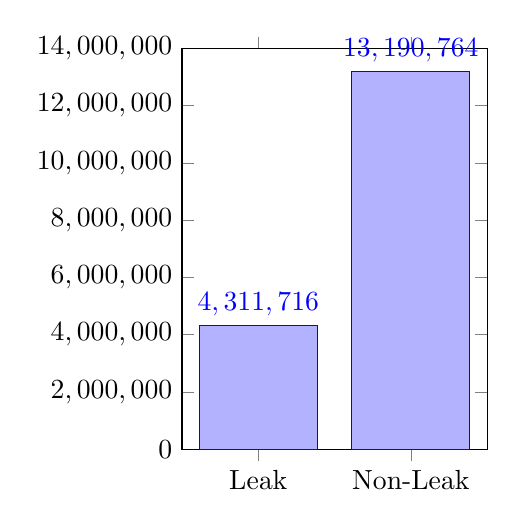
\begin{tikzpicture}
\begin{axis}[
    ybar,
    bar width=1.5cm,
    width=0.45\textwidth,
    height=0.55\textwidth,
    symbolic x coords={Leak, Non-Leak},
    xtick=data,
    ymin=0,
    ymax=14000000,
    ytick={0,2000000,4000000,6000000,8000000,10000000,12000000,14000000},
    scaled y ticks=false,
    yticklabel style={
        /pgf/number format/fixed,
        /pgf/number format/precision=0,
        /pgf/number format/1000 sep={,}
    },
    nodes near coords,
    nodes near coords style={
        /pgf/number format/fixed,
        /pgf/number format/precision=0,
        /pgf/number format/1000 sep={,}
    },
    enlarge x limits=0.5,
]
\addplot coordinates {(Leak,4311716) (Non-Leak,13190764)};
\end{axis}
\end{tikzpicture}
\caption{Distribution of leak and non-leak rows in the dataset.}
\label{fig:leak_distribution}
\end{figure}

A scenario that has at least one leak state is called a \textit{leak scenario}, while one with no leak state at any timestamp is called a \textit{non-leak scenario}. Out of the 999 scenarios, 758 are \textit{leak scenarios}, while 241 are \textit{non\_leak scenarios}. This ratio is also maintained while selecting the scenarios for training, validation, and testing.

\vspace{0.3cm}
Below is the distribution of leak instances across nodes from 0-31 (32 nodes).

\begin{figure}[H]
    \centering
    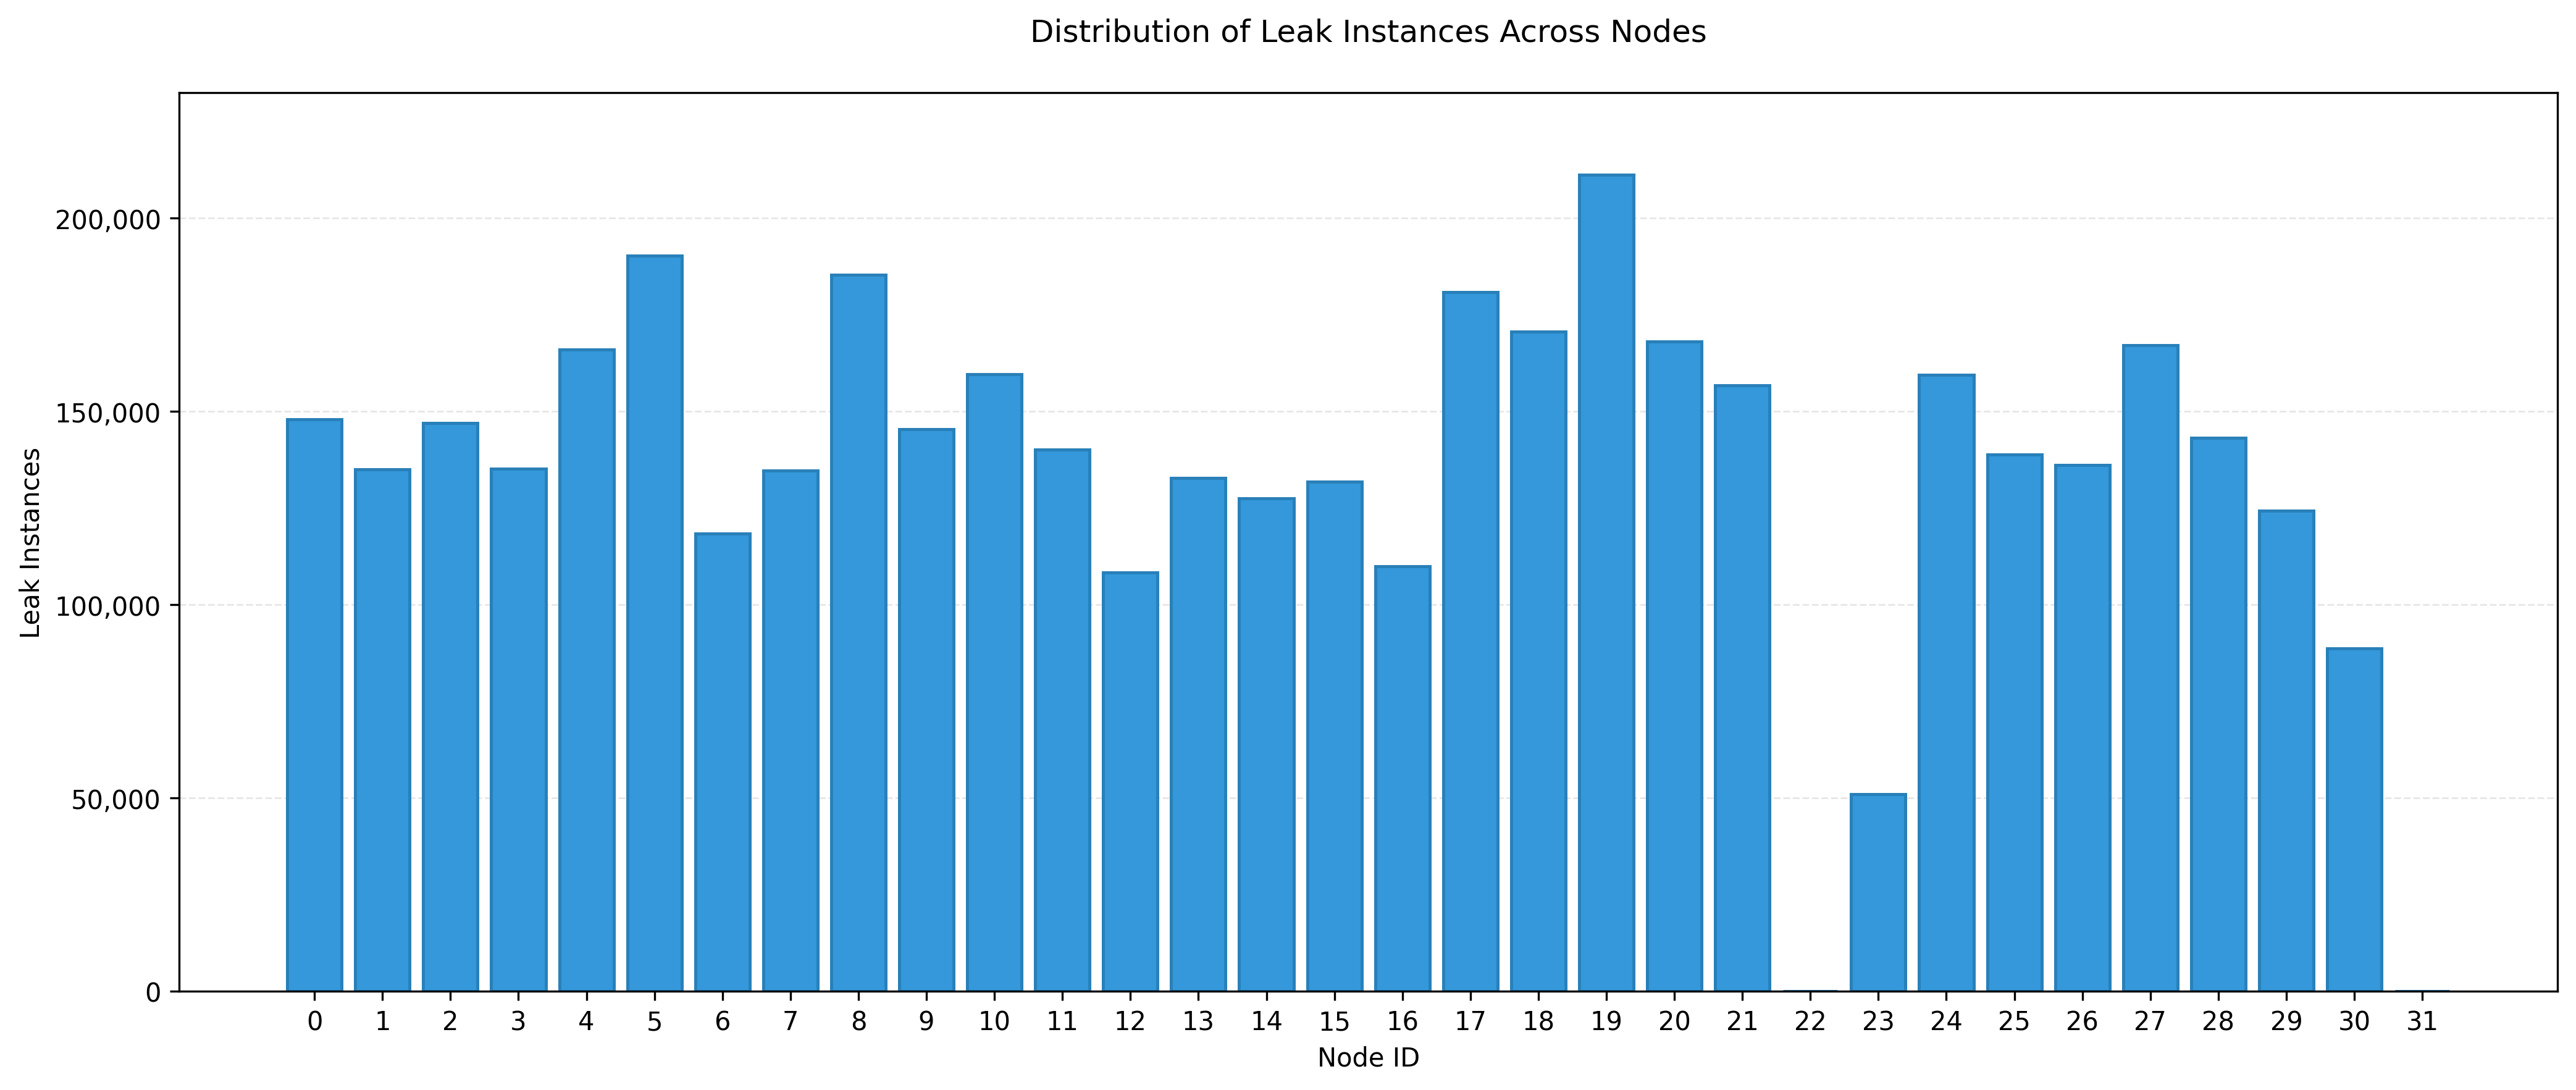
\includegraphics[width=1.1\linewidth]{leak_instances_bar.png}
    \caption{Distribution of leak instances for all scenarios across nodes.}
    \label{fig:leak_instances}
\end{figure}

As we can see, node 19 has the highest leak instances, while node 22 and node 31 have no leaks. Using this, the rule-based system can be programmed to be biased more towards some nodes than others, to improve node localization accuracy.

\subsection{Feature Engineering and Pre-Processing}

In terms of feature engineering, two features have been added to each scenario for an increase in model performance. As the data does not have any missing or \textit{NaN} values, filling in missing data is not needed and only data normalization has been performed in terms of pre-processing.

\subsubsection{Adding columns}

During daytime, due to usage of water both commercial and industrial, the general trend of pressure and flow is downward, while demand is higher and and the reverse at night. In order to prevent the models from reading the downward trend of pressure and flow and keep returning leak predictions, two columns, \textit{sin\_hour} and \textit{cos\_hour}, are added to each scenario, in order to add weight to the particular hour of the day when a leak occurs. 

Let $i$ denote the row index of a scenario. The \textit{step of day} $s$ is defined as:
\[
s_i = i \bmod 48
\]

The temporal features are described as:
\[
\text{sin\_hour}_i = \sin\!\left( \frac{2\pi s_i}{48} \right)
\]

\[
\text{cos\_hour}_i = \cos\!\left( \frac{2\pi s_i}{48} \right)
\]

Because of these columns, a time step of 12 A.M. (sin\_hour = 0 and cos\_hour = 1) is given more bias by the model for a positive classification than 9 A.M. (sin\_hour = 0.707 and cos\_hour = -0.707) for similar readings of pressure, demand and flow.

\subsubsection{Normalization}

All sets (train, validation, and test) are normalized using the mean and standard deviation of the training set, such that the mean of each set is 0 and the standard deviation is 1, after normalization.

\vspace{0.05cm}

Let $\mathcal{D}_{\text{train}} = \{\mathbf{x}_1, \mathbf{x}_2, \dots, \mathbf{x}_N\}$
denote the training dataset, where each feature vector
$\mathbf{x}_i \in \mathbb{R}^{F}$.

The global mean and standard deviation are computed feature-wise over the
training set as:
\begin{equation}
\boldsymbol{\mu} =
\frac{1}{N} \sum_{i=1}^{N} \mathbf{x}_i,
\end{equation}

\begin{equation}
\boldsymbol{\sigma} =
\sqrt{
\frac{1}{N} \sum_{i=1}^{N} \mathbf{x}_i^{\circ 2}
- \boldsymbol{\mu}^{\circ 2}
},
\end{equation}
where $\circ$ denotes element-wise operations.

To ensure numerical stability, the variance is lower bounded by a small constant
$\epsilon$:
\begin{equation}
\boldsymbol{\sigma} =
\sqrt{
\max\left(
\frac{1}{N} \sum_{i=1}^{N} \mathbf{x}_i^{\circ 2}
- \boldsymbol{\mu}^{\circ 2},
\epsilon
\right)
}.
\end{equation}

Using the statistics computed from the training set, each feature is normalized
as:
\begin{equation}
\tilde{\mathbf{x}} =
\frac{\mathbf{x} - \boldsymbol{\mu}}{\boldsymbol{\sigma}},
\end{equation}
where $\tilde{\mathbf{x}}$ denotes the normalized feature vector.

The same training-set mean $\boldsymbol{\mu}$ and standard deviation
$\boldsymbol{\sigma}$ are applied consistently to the training, validation, and
test sets to avoid data leakage.

\subsection{Windowing function}

To give the model temporal context and features without the use of recurrent architectures such as LSTMs or GRUs, a sliding-window dataset construction is used. Temporal windows are extracted from each scenario using a fixed window size of $12$, or 6 hours as each time-step is 30 minutes. For each window, the target is the leak state (0/1) at the final time stamp of the window, allowing the model to learn temporal patterns preceding a leak event. As the target label is the leak state at the final time stamp, which is also the current time stamp, this means that the model \textbf{nowcasts} leakage prediction. 

\subsubsection{ANN}

For the ANN models (base ANN and Physics-Aware ANN), each window is flattened into a one-dimensional vector as input to the network. A window of 12 time stamps with 100 features per time stamp is reshaped into a vector of dimension one and length $12\times100$. The mathematical representation is:

Let a scenario be represented as a multivariate time series
\begin{equation}
\mathbf{X} = \{\mathbf{x}_1, \mathbf{x}_2, \dots, \mathbf{x}_T\},
\quad
\mathbf{x}_t \in \mathbb{R}^{F},
\end{equation}
where $F$ denotes the number of features at each time step.

Using a sliding window of length $W$, the $k$-th temporal window is defined as
\begin{equation}
\mathbf{X}^{(k)} =
\left[
\mathbf{x}_{k},
\mathbf{x}_{k+1},
\dots,
\mathbf{x}_{k+W-1}
\right]
\in \mathbb{R}^{W \times F}.
\end{equation}

For the ANN model, each window is reshaped into a one-dimensional feature vector via vectorization:
\begin{equation}
\tilde{\mathbf{x}}^{(k)} =
\mathrm{vec}\left(\mathbf{X}^{(k)}\right)
\in \mathbb{R}^{W \cdot F}.
\end{equation}

This flattened representation serves as the input to the fully connected network.

\section{Physics Loss}

Water distribution networks are governed by conservation of mass and energy. Our physics loss enforces these laws. The network is modeled as a directed graph, where vertices represent nodes, and edges represent pipes connecting nodes. \textit{Mass conservation} is enforced at each node, and \textit{Energy conservation} is enforced along each pipe. The equations used for these are discussed below.

\subsection{Equations}
For \textit{Mass conservation}, the \textbf{Continuity Equation} is used. This means that the inflow at each node is equal to the sum of the demand at that node and the outflow at each node.
\[
r^{(i)}_{\mathrm{mass}}
=
\sum_{j \in \mathcal{E}_{\mathrm{in}}(i)} Q_j
-
\sum_{j \in \mathcal{E}_{\mathrm{out}}(i)} Q_j
-
D_i,
\]
where $Q_j$ denotes the flow through pipe $j$, $D_i$ is the demand, and $\mathcal{E}_{\mathrm{in}}(i)$ and $\mathcal{E}_{\mathrm{out}}(i)$ represent incoming and outgoing pipes, respectively.

\vspace{0.3cm}

For \textit{Energy conservation}, the \textit{Hazen-Williams Equation} is used. The \textbf{Hazen-Williams Equation} defines the loss due to friction in a pipe; this frictional loss, along with the elevation head differences between the two ends of a pipe, gives the pressure drop. Since in the LeakDB dataset, in all scenarios, all nodes are kept at the same elevation, the pressure drop due to elevation differences is assumed to be negligible. The Hazen-Williams head loss for pipe $k$ is given by
\[
h_k
=
10.67 \frac{L_k |Q_k|^{1.852}}{C_k^{1.852} D_k^{4.87}},
\]
where $L_k$ is the pipe length, $D_k$ is the diameter, $C_k$ is the roughness coefficient, and $Q_k$ is the predicted flow.

\subsection{Physics Loss Algorithm}
The physics loss due to mass conservation is defined as:
\[
\mathcal{L}_{\mathrm{mass}}
=
\frac{1}{N} \sum_{i=1}^{N} \left( \frac{r^{(i)}_{\mathrm{mass}}}{\bar{D}} \right)^2,
\]
where $\bar{D}$ denotes a scale factor (e.g., mean absolute demand) for numerical stability.

The predicted pressure drop across a pipe is given as:
\[
\Delta p_k
=
\operatorname{sign}(Q_k) \left( p_{\mathrm{src}(k)} - p_{\mathrm{dst}(k)} \right),
\]
where $p_{\mathrm{src}(k)}$ and $p_{\mathrm{dst}(k)}$ are the predicted pressures at the source and destination nodes.

Thus, the loss due to energy conservation is defined as:
\[
r^{(k)}_{\mathrm{energy}}
=
\Delta p_k - h_k,
\]
\[
\mathcal{L}_{\mathrm{energy}}
=
\frac{1}{M} \sum_{k=1}^{M} \left( \frac{r^{(k)}_{\mathrm{energy}}}{\bar{p}} \right)^2,
\]
where $\bar{p}$ denotes a scale factor (e.g., mean absolute predicted pressure) for numerical stability.

The total physics loss is a weighted average of the loss due to mass conservation and energy conservation, given as:
\[
\mathcal{L}_{\mathrm{phys}}
=
\lambda_{\mathrm{mass}} \mathcal{L}_{\mathrm{mass}}
+
\lambda_{\mathrm{energy}} \mathcal{L}_{\mathrm{energy}},
\]
where $\lambda_{\mathrm{mass}}$ and $\lambda_{\mathrm{energy}}$ are hyperparameters; in our implementation we use $\lambda_{\mathrm{mass}} = 1.0$ and $\lambda_{\mathrm{energy}} = 0.1$ to emphasize mass conservation consistency.

\subsection{Pseudocode and Training Integration}

Algorithm~\ref{alg:physics_loss} computes the physics loss given model predictions and pipe parameters. Algorithm~\ref{alg:training} shows how it is integrated into the Physics-Aware ANN training loop. Predictions are denormalized before the physics loss is evaluated, since the conservation laws apply in physical units.

\noindent\textbf{Algorithm 1: Physics Loss}
\label{alg:physics_loss}

\small
\noindent\textit{Input:} $\hat{p}$ (pred. pressure), $\hat{Q}$ (pred. flow), $D$ (demand), $L,D,C$ (pipe params), $\mathsf{edge\_index}$

\noindent\textit{Output:} $\mathcal{L}_{\mathrm{phys}}$, $\mathcal{L}_{\mathrm{total}}$

\begin{enumerate}
    \item Aggregate flow at nodes: $\mathsf{flow\_in}[i] \leftarrow \sum_{j:\mathsf{dst}(j)=i} \hat{Q}_j$, $\mathsf{flow\_out}[i] \leftarrow \sum_{j:\mathsf{src}(j)=i} \hat{Q}_j$
    \item Mass residual: $r^{(i)}_{\mathrm{mass}} \leftarrow \mathsf{flow\_in}[i] - \mathsf{flow\_out}[i] - D_i$
    \item $\mathcal{L}_{\mathrm{mass}} \leftarrow \mathrm{mean}\bigl((r_{\mathrm{mass}} / \bar{D})^2\bigr)$
    \item Hazen-Williams head loss: $h_k \leftarrow 10.67 \cdot L_k |\hat{Q}_k|^{1.852} / (C_k^{1.852} D_k^{4.87})$
    \item Predicted pressure drop: $\Delta p_k \leftarrow \mathsf{sign}(\hat{Q}_k) \cdot (\hat{p}_{\mathsf{src}(k)} - \hat{p}_{\mathsf{dst}(k)})$
    \item Energy residual: $r^{(k)}_{\mathrm{energy}} \leftarrow \Delta p_k - h_k$
    \item $\mathcal{L}_{\mathrm{energy}} \leftarrow \mathrm{mean}\bigl((r_{\mathrm{energy}} / \bar{p})^2\bigr)$
    \item $\mathcal{L}_{\mathrm{phys}} \leftarrow \lambda_{\mathrm{mass}} \mathcal{L}_{\mathrm{mass}} + \lambda_{\mathrm{energy}} \mathcal{L}_{\mathrm{energy}}$
    \item $\mathcal{L}_{\mathrm{total}} \leftarrow \mathcal{L}_{\mathrm{WBCE}} + \lambda_{\mathrm{phys}} \mathcal{L}_{\mathrm{phys}}$
\end{enumerate}

\vspace{0.3em}
\noindent\textbf{Algorithm 2: Training Loop with Physics Loss}
\label{alg:training}

\begin{enumerate}
    \item Set $\lambda_{\mathrm{phys}}$ by epoch: $0.01$ if $e < 10$, $0.03$ if $10 \le e < 20$, else $0.05$
    \item For each batch $(x_b, y_b, \mathsf{scenario\_ids}, D_b)$:
    \begin{enumerate}
        \item Load pipe params $(L, D, C)$ for each scenario in batch
        \item Denormalize $D_b$ to physical units
        \item Forward: $(\hat{y}, \hat{p}, \hat{Q}) \leftarrow \mathsf{model}(x_b)$
        \item Denormalize $\hat{p}$, $\hat{Q}$ to physical units
        \item $\mathcal{L}_{\mathrm{WBCE}} \leftarrow \mathsf{weighted\_BCE}(\hat{y}, y_b)$
        \item $\mathcal{L}_{\mathrm{total}} \leftarrow \mathsf{PhysicsLoss}(\mathcal{L}_{\mathrm{WBCE}}, \hat{p}, \hat{Q}, D_b, L, D, C, \mathsf{edge\_index}, \lambda_{\mathrm{phys}})$
        \item Backpropagate $\mathcal{L}_{\mathrm{total}}$, update parameters
    \end{enumerate}
\end{enumerate}

\normalsize

\subsection{Integration into Model}
To use this loss in the Physics-Aware ANN model, the \textit{.inp} files of each scenario are formatted into a \textit{.csv} file containing the pipe length, diameter, and roughness coefficient of each pipe in the scenario, and this information is integrated into the dataset class. As the node-pipe connection is constant for all scenarios, a constant \textit{edge\_list} is created and used. During training, the physics loss is added to the classification loss, and the combined loss is used for backpropagation.

\subsection{The Thought}
The physics loss constrains the model's latent space so that predictions remain physically plausible and do not violate conservation laws. Over training, the residuals between true and predicted pressure and flow decrease. The predicted pressure and flow values are also fed into the leak classification head, as described in the model architecture section.

\section{Model Architecture and Training Details}

\subsection{Architecture}

\subsubsection{Base ANN Model}

The base ANN is a fully connected feed-forward network designed for binary classification of leak presence at a single timestamp. The input layer consists of 1200 features, from the windowing preprocessing. It is passed through three hidden layers of 512, 256 and 64 neurons. The first two hidden layers employ Batch Normalization and ReLU activation, and dropout (rate $= 0.5$) to prevent overfitting. The third hidden layer uses only ReLU activation. The output layer consists of a single neuron with a sigmoid activation function, for binary leak classification.

\vspace{0.5cm}

\textbf{ANN Loss: }

As discussed above, because the model is a binary classification model, and the class imbalance is severe, \textbf{Class-weighted binary cross-entropy} loss is used, where the loss is reweighted inversely proportional to class frequency.

Let \(N_0\) denote the number of non-leak samples, and  
let \(N_1\) denote the number of leak samples.

\[
w_0 = \frac{N_0 + N_1}{2 N_0}, \qquad
w_1 = \frac{N_0 + N_1}{2 N_1}
\]

Let \(y_i \in \{0,1\}\) denote the ground-truth leak label for the \(i\)-th sample,  
and let \(\hat{y}_i \in (0,1)\) denote the corresponding predicted leak probability.

\[
\mathcal{L}_{\text{WBCE}}
= - \frac{1}{N} \sum_{i=1}^{N}
\left[
w_1 \, y_i \log(\hat{y}_i)
+ w_0 \, (1 - y_i) \log(1 - \hat{y}_i)
\right]
\]

\begin{figure}[H]
    \centering
    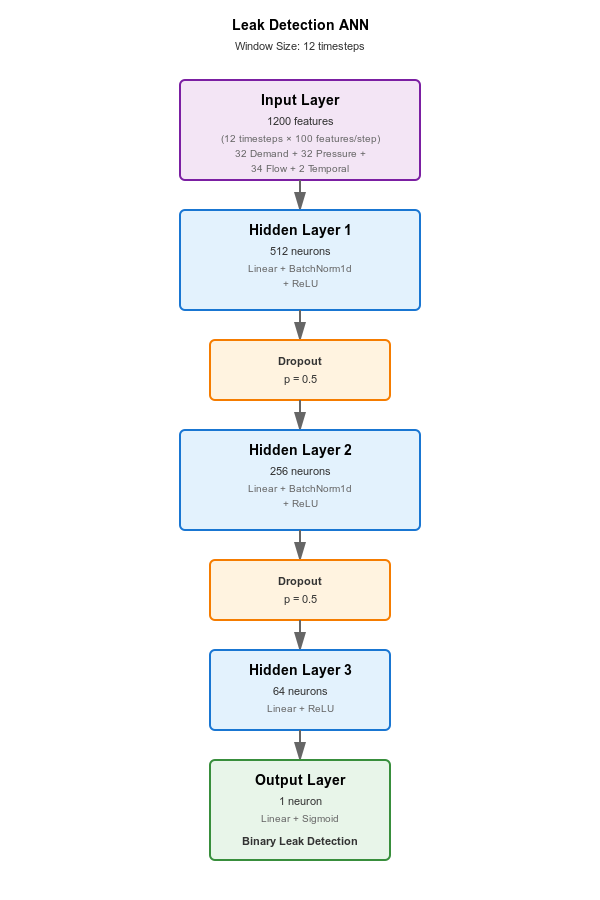
\includegraphics[width=\linewidth]{ann_architecture (1).png}
    \caption{Architecture Diagram of ANN}
    \vspace{0.05cm}
    \label{fig:architecture_diagram}
\end{figure}

\subsubsection{Physics-Aware ANN Model}

The Physics-Aware ANN is a fully connected feed-forward network designed for joint prediction of pressure and flow, and classification of leak presence on a single timestamp using those predictions. The input layer receives 1200 features (window size $\times$ features per timestep). The network comprises three hidden layers of 512, 256, and 64 neurons. The first two hidden layers employ Batch Normalization, ReLU activation, and Dropout (rate $= 0.5$); the third hidden layer uses Batch Normalization and ReLU only. From the third hidden layer, two auxiliary heads branch out: a pressure head with 32 output neurons (one per node) and a flow head with 34 output neurons (one per pipe). The leak classification head takes as input the concatenation of the 64-dimensional representation from the third hidden layer and 5 physics-derived features: mean pressure, standard deviation of pressure, range of pressure (max $-$ min), mean flow, and standard deviation of flow—yielding 69 features in total. These are passed through a hidden layer of 64 neurons with ReLU and Dropout, followed by a single output neuron with sigmoid activation for binary leak classification.

\vspace{0.5cm}

\textbf{Physics-Aware ANN Loss: }

The \textbf{Class-weighted binary cross-entropy}, also the \textbf{Classification loss} of the model is given by:

Let \(N_0\) denote the number of non-leak samples, and  
let \(N_1\) denote the number of leak samples.

\[
w_0 = \frac{N_0 + N_1}{2 N_0}, \qquad
w_1 = \frac{N_0 + N_1}{2 N_1}
\]

Let \(y_i \in \{0,1\}\) denote the ground-truth leak label for the \(i\)-th sample,  
and let \(\hat{y}_i \in (0,1)\) denote the corresponding predicted leak probability.

\[
\mathcal{L}_{\text{WBCE}}
= - \frac{1}{N} \sum_{i=1}^{N}
\left[
w_1 \, y_i \log(\hat{y}_i)
+ w_0 \, (1 - y_i) \log(1 - \hat{y}_i)
\right]
\]

Let the physics loss described above be denoted by
$\mathcal{L}_{\mathrm{phys}}$

Thus, the total loss of the model is given by:
\[
\mathcal{L}_{\mathrm{total}}
=
\mathcal{L}_{\mathrm{WBCE}}
+
\lambda_{\mathrm{phys}} \, \mathcal{L}_{\mathrm{phys}}.
\]

The coefficient $\lambda_{\mathrm{phys}}$ follows a warm-up schedule across training epochs $e$:
\[
\lambda_{\mathrm{phys}}(e)
=
\begin{cases}
0.01, & e < 10, \\
0.03, & 10 \le e < 20, \\
0.05, & e \ge 20.
\end{cases}
\]

This schedule ensures that the physics loss does not dominate the classification loss in early training, allowing the model to first learn discriminative patterns before enforcing physical consistency.

\begin{figure}[H]
    \centering
    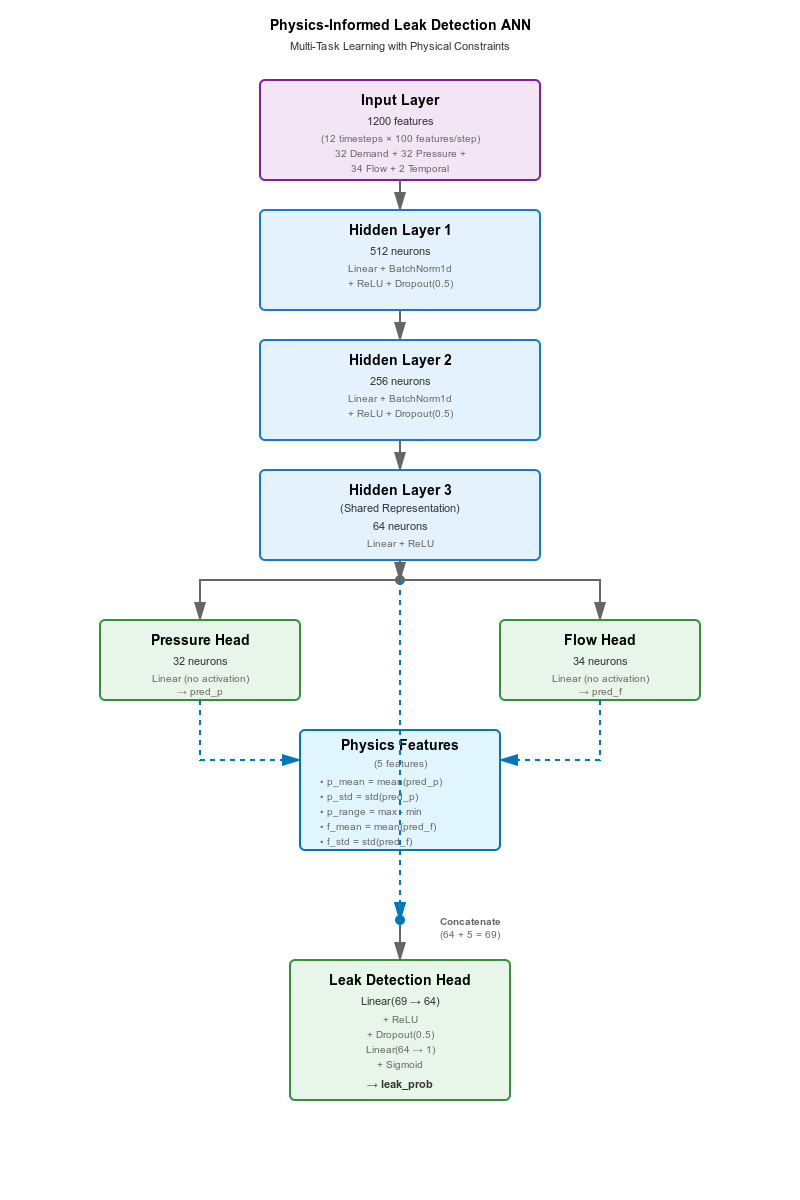
\includegraphics[width=1.05\linewidth]{physics_ann_architecture (2).png}
    \caption{Architecture Diagram of Physics-Aware ANN}
    \vspace{0.05cm}
    \label{fig:architecture_diagram}
\end{figure}

\subsection{Training strategy and Hyper-parameters}

\section{Localization}

\subsection{Introduction}

\subsection{Algorithm}

\subsection{Metrics}

\section{Results and Discussion}

\subsection{Metrics}

We use four standard metrics: \textbf{Accuracy}, \textbf{Precision}, \textbf{Recall}, and \textbf{F1-Score} to evaluate the performance of our classification models.
\vspace{0.1cm}
Accuracy measures the overall ratio of correctly classified instances.
\begin{align}
    \text{Accuracy} &= \frac{TP + TN}{TP + TN + FP + FN} \\[6pt]
\end{align}
Precision measures how many positive predictions are also true positives.
\begin{align}
    \text{Precision} &= \frac{TP}{TP + FP} \\[6pt]
\end{align}
Recall measures how many of the true positives are actually predicted as true.
\begin{align}
    \text{Recall} &= \frac{TP}{TP + FN} \\[6pt]
\end{align}
F1-score is a harmonic mean of the Precision and Recall, acting as a single number that tells us about the performance of any model.
\begin{align}
    \text{F1-score} &= 2 \times \frac{\text{Precision} \times \text{Recall}}{\text{Precision} + \text{Recall}}
\end{align}

\subsection{Base Model Performance}

Both the base ANN and Physics-Aware ANN are trained on 490 scenarios, with the validation and test sets comprising 105 scenarios each. Each model is trained for 30 epochs, and the model checkpoint with the highest validation F1 is used for testing. Both models are evaluated at a classification threshold of \textbf{0.5}.

Highest Validation F1 for the base ANN model is \textbf{0.7483}.

\subsubsection{ANN}

\vspace{0.03cm}

\textbf{Model Metrics:}

\begin{table}[H]
\begin{tabular}{@{}lllll@{}}
\toprule
\textbf{Accuracy} & \textbf{Precision} & \textbf{Recall} & \textbf{F1} \\ \midrule
0.9213       & 0.9143         & 0.7889      & 0.8470      
\end{tabular}
\end{table}

\textbf{Confusion Matrix:}

\begin{table}[H]
\centering
\label{tab:conf_matrix}
\begin{tabular}{lcc}
\toprule
 & \textbf{Predicted No Leak} & \textbf{Predicted Leak} \\
\midrule
\textbf{Actual No Leak} & 1293741 & 37515 \\
\textbf{Actual  Leak} & 107085 & 400104 \\
\bottomrule
\end{tabular}
\end{table}

\textbf{Plot of Val F1 vs Epochs:}

\begin{figure}[H]
\centering
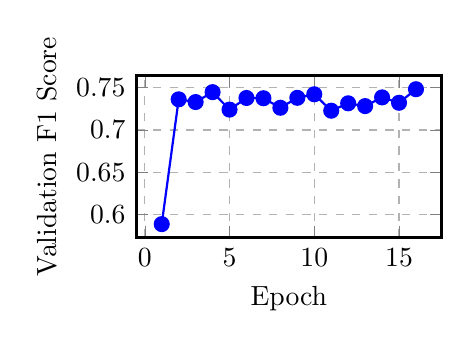
\begin{tikzpicture}
\begin{axis}[
    width=0.45\textwidth,
    height=0.3\textwidth,
    xlabel={Epoch},
    ylabel={Validation F1 Score},
    grid=major,
    grid style={dashed, black!30},
    legend pos=south east,
    mark size=2.5pt,
    line width=1.2pt,
    every axis plot/.append style={thick}
]

\addplot[
    color=blue,
    mark=*,
    thick,
] coordinates {
    (1, 0.5884)
    (2, 0.7363)
    (3, 0.7331)
    (4, 0.7448)
    (5, 0.7241)
    (6, 0.7379)
    (7, 0.7376)
    (8, 0.7263)
    (9, 0.7381)
    (10, 0.7423)
    (11, 0.7228)
    (12, 0.7316)
    (13, 0.7283)
    (14, 0.7386)
    (15, 0.7322)
    (16, 0.7483)
};

\end{axis}
\end{tikzpicture}
\caption{Validation F1 score across training epochs for ANN}
\label{fig:val_f1}
\end{figure}

\subsection{Physics-Aware Model Performance}

The Physics-Aware ANN is trained under the same data split and evaluation protocol as the base ANN (490 train, 105 validation, 105 test scenarios; 30 epochs; threshold 0.5).

Highest Validation F1 for the Physics-Aware ANN is \textbf{0.7549}.

\vspace{0.03cm}

\textbf{Model Metrics:}

\begin{table}[H]
\begin{tabular}{@{}lllll@{}}
\toprule
\textbf{Accuracy} & \textbf{Precision} & \textbf{Recall} & \textbf{F1} \\ \midrule
0.9303       & 0.9659        & 0.7747      & 0.8598     
\end{tabular}
\end{table}

\textbf{Confusion Matrix:}

\begin{table}[H]
\centering
\label{tab:conf_matrix}
\begin{tabular}{lcc}
\toprule
 & \textbf{Predicted No Leak} & \textbf{Predicted Leak} \\
\midrule
\textbf{Actual No Leak} & 1317369 & 13887 \\
\textbf{Actual  Leak} & 114272 & 392917 \\
\bottomrule
\end{tabular}
\end{table}

\textbf{Plot of Val F1 vs Epochs:}

\begin{figure}[H]
\centering
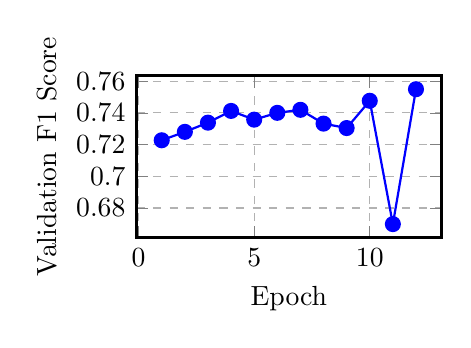
\begin{tikzpicture}
\begin{axis}[
    width=0.45\textwidth,
    height=0.3\textwidth,
    xlabel={Epoch},
    ylabel={Validation F1 Score},
    grid=major,
    grid style={dashed, black!30},
    legend pos=south east,
    mark size=2.5pt,
    line width=1.2pt,
    every axis plot/.append style={thick}
]

\addplot[
    color=blue,
    mark=*,
] coordinates {
    (1, 0.7227)
    (2, 0.7280)
    (3, 0.7338)
    (4, 0.7412)
    (5, 0.7357)
    (6, 0.7400)
    (7, 0.7419)
    (8, 0.7332)
    (9, 0.7304)
    (10, 0.7476)
    (11, 0.6698)
    (12, 0.7549)
};

\end{axis}
\end{tikzpicture}
\caption{Validation F1 score across training epochs for Physics-Aware ANN}
\label{fig:val_f1_paann}
\end{figure}

\subsection{Comparison among models and existing Benchmarks}

\textbf{Comparison between ANN and Physics-Aware ANN:}

\begin{table}[H]
\centering
\begin{tabular}{@{}llllll@{}}
\toprule
\textbf{Model}             & \textbf{Accuracy} & \textbf{Precision} & \textbf{Recall} & \textbf{F1}     \\ \midrule
ANN               & 0.9213   & 0.9143    & \textbf{0.7889} & 0.8470 \\
Physics-Aware ANN & \textbf{0.9303}   & \textbf{0.9659}    & 0.7747 & \textbf{0.8598}  
\end{tabular}
\end{table}

The Physics-Aware ANN gets an improvement of 0.98\% in accuracy, 5.64\% in precision, and 1.51\% in F1 compared to the ANN, while having a decrease of 1.79\% in recall. The Physics-Aware ANN reduces the number of false positives by 23,628 (62.98\% reduction), at the cost of increasing the false negatives by 7,187 (6.71\% increase). This indicates that the Physics-Aware ANN is more conservative while predicting leaks, issuing leak predictions only when they are physically consistent and more confident than the ANN, which has a more liberal behavior while predicting leaks.

In practical deployment, this trade-off means that the Physics-Aware ANN may incur a slight delay in detecting certain leak events; however, it also drastically lowers the number of false alarms, resulting in a significant reduction of unnecessary human intervention and monetary costs.

\section{Why Classical Machine Learning Techniques Are Not Used}

To assess whether classical machine learning methods could suffice for leak detection, we trained XGBoost classifiers on the same windowed dataset. Table~\ref{tab:xgboost} summarizes the results for $N$-estimators $= 50$ and $100$, evaluated at threshold 0.5 and at the optimal threshold (ROC curve–derived, approximately 0.44). While XGBoost performs reasonably, it lags behind both the base ANN (F1 0.8470) and the Physics-Aware ANN (F1 0.8598). More importantly, XGBoost is purely data-driven and does not incorporate conservation of mass and energy. As a result, it cannot guarantee physically consistent predictions and tends toward higher false positive rates. The Physics-Aware ANN, by embedding hydraulic constraints into the loss, achieves better precision and lower false positives while maintaining strong recall, making it preferable for operational deployment.

\begin{table}[H]
\centering
\caption{XGBoost on LeakDB Hanoi. $N$: trees; Thr.: threshold. ROC-AUC: 0.8705 ($N$=50), 0.8752 ($N$=100).}
\label{tab:xgboost}
\small
\resizebox{\columnwidth}{!}{%
\begin{tabular}{@{}ccrrrr@{}}
\toprule
\textbf{$N$} & \textbf{Thr.} & \textbf{Acc.} & \textbf{Prec.} & \textbf{Rec.} & \textbf{F1} \\ \midrule
50  & 0.50   & 0.8959 & 0.9519 & 0.6557 & 0.7765 \\
50  & 0.44   & 0.8183 & 0.8695 & 0.7003 & 0.7758 \\
100 & 0.50   & 0.9042 & 0.9567 & 0.6836 & 0.7974 \\
100 & 0.44   & 0.8249 & 0.8905 & 0.7141 & 0.7926 \\ \bottomrule
\end{tabular}%
}
\end{table}

\section{Validity of Loss Function}

\begin{figure}[H]
\centering
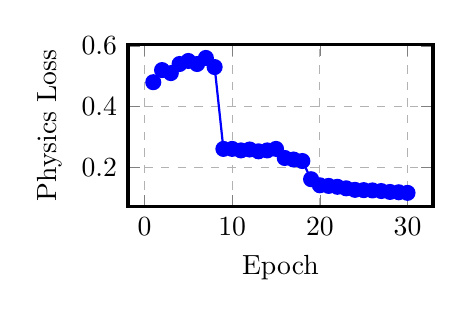
\begin{tikzpicture}
\begin{axis}[
    width=0.45\textwidth,
    height=0.3\textwidth,
    xlabel={Epoch},
    ylabel={Physics Loss},
    grid=major,
    grid style={dashed, black!30},
    legend pos=north east,
    mark size=2.5pt,
    line width=1.2pt,
    every axis plot/.append style={thick}
]

\addplot[
    color=blue,
    mark=*,
] coordinates {
    (1, 0.48)
    (2, 0.52)
    (3, 0.51)
    (4, 0.54)
    (5, 0.55)
    (6, 0.54)
    (7, 0.56)
    (8, 0.53)
    (9, 0.26)
    (10, 0.26)
    (11, 0.255)
    (12, 0.258)
    (13, 0.252)
    (14, 0.255)
    (15, 0.26)
    (16, 0.23)
    (17, 0.225)
    (18, 0.22)
    (19, 0.16)
    (20, 0.14)
    (21, 0.138)
    (22, 0.135)
    (23, 0.13)
    (24, 0.125)
    (25, 0.124)
    (26, 0.123)
    (27, 0.121)
    (28, 0.118)
    (29, 0.117)
    (30, 0.115)
};

\end{axis}
\end{tikzpicture}
\caption{Physics loss convergence across training epochs}
\label{fig:physics_loss}
\end{figure}

A valid loss function should exhibit a decreasing trend during training when the model learns the objective. Similarly to how the weighted BCE loss decreases as the model learns classification, the physics loss of the Physics-Aware ANN decreases as it learns the underlying physics and the predicted pressure and flow values yield smaller residuals over epochs.

\section{Sensitivity Analysis}

To assess model robustness under distribution shift, we conduct a sensitivity analysis that simulates changes in operational conditions. Population growth or decline affects water demand, which in turn alters pressure and flow throughout the network. We perturb the test set to simulate demand shifts of $\pm 5\%$, $\pm 10\%$, and $\pm 15\%$, and correspondingly adjust pressure and flow.

\subsection{Methodology}

For each perturbation level $\alpha \in \{-0.15, -0.10, -0.05, 0, 0.05, 0.10, 0.15\}$ (e.g., $\alpha = 0.10$ corresponds to a 10\% increase in demand):

\begin{itemize}
    \item \textbf{Demand:} $D' = D \cdot (1 + \alpha)$, where $D$ is the original demand.
    \item \textbf{Flow:} Flow scales approximately with demand; we set $Q' = Q \cdot (1 + \alpha)$.
    \item \textbf{Pressure:} Pressure typically decreases when demand increases (and vice versa). We use $p' = p \cdot (1 - \beta \alpha)$, where $\beta \in (0,1]$ is a coupling coefficient. We use $\beta = 0.7$ to reflect the pressure--demand relationship.
\end{itemize}

The perturbed test set is normalized using the same training-set statistics as the original data. The trained base ANN and Physics-Aware ANN are evaluated on these perturbed test sets without retraining. This evaluates how well the models generalize when operational conditions deviate from the training distribution.

\subsection{Results}

Table~\ref{tab:sensitivity} summarizes the F1 score of both models across perturbation levels. The baseline ($\alpha = 0$) is included for reference. As $\alpha$ deviates from zero, some degradation in F1 is expected; the Physics-Aware ANN is expected to degrade more gracefully due to its incorporation of conservation laws, which remain valid under demand scaling.

\begin{table}[H]
\centering
\caption{Sensitivity analysis: F1 under demand perturbation. $\alpha$: demand change; $\alpha=0$ unperturbed.}
\label{tab:sensitivity}
\small
\resizebox{\columnwidth}{!}{%
\begin{tabular}{@{}lrrrrrrr@{}}
\toprule
\textbf{Model} & $-15\%$ & $-10\%$ & $-5\%$ & $0\%$ & $+5\%$ & $+10\%$ & $+15\%$ \\ \midrule
ANN & -- & -- & -- & 0.847 & -- & -- & -- \\
PAANN & -- & -- & -- & 0.860 & -- & -- & -- \\ \bottomrule
\end{tabular}%
}
\end{table}

\section{Localization Results}

\subsection{Quantitative Results}

\subsection{Qualitative Results}

\subsection{Comparison with Baselines}

\section{Limitations}

Experiments were conducted on the LeakDB Hanoi benchmark, a widely used simulated dataset that allows controlled, reproducible evaluation. The Hanoi network (32 nodes, 34 pipes) serves as a standard testbed in the leak-detection literature. Training leveraged cloud compute for efficiency. The sensitivity analysis employs a tractable pressure–demand coupling to explore robustness under demand shifts; future work may incorporate full hydraulic simulation for finer-grained perturbation modeling.
\section{Conclusion}

We presented a Physics-Aware Artificial Neural Network (PAANN) for leak detection in Water Distribution Networks, embedding conservation of mass and the Hazen-Williams relation into the training objective. Experiments on the LeakDB Hanoi dataset show that the Physics-Aware ANN outperforms both a base ANN and XGBoost, achieving an F1 score of 0.8598 with a 62.98\% reduction in false positives compared to the base ANN. By enforcing physical consistency, the model issues leak predictions only when they are hydraulically plausible, reducing false alarms and operational costs. We also introduced a sensitivity analysis framework to assess robustness under demand perturbations and discussed why classical machine learning methods such as XGBoost are less suitable for this task. Our results demonstrate that incorporating domain physics into neural network training improves detection reliability and supports the case for physics-aware approaches in critical infrastructure monitoring.

\section{Future Work}

Natural extensions include applying the Physics-Aware ANN to additional LeakDB topologies (e.g., Net1) and real-world SCADA datasets, incorporating EPANET-based perturbations in the sensitivity analysis, and exploring hybrid graph–physics architectures for larger networks. The rule-based localization component can be extended and benchmarked against alternative approaches. These directions build on the physics-aware framework presented here.

\section{Acknowledgements}
Each member of this group has contributed equally and with the same sense of enthusiasm and ownership for this project.
\newline We would like to acknowledge Prof. Abhijeet Salunke for his mentorship, guidance and constant encouragement across the entire journey of the project.
\newline We would also like to acknowledge Prof. Vasan Arunachalam from BITS Pilani, Hyderabad campus for clarifying our questions regarding the LeakDB dataset. 
\section{Appendix}

\subsection{Ablation Studies}

We report ablations on three design choices: window size, temporal columns, and the physics-aware mechanism. All ablations use the base ANN unless otherwise noted; the physics-aware mechanism ablation compares two variants of the Physics-Aware ANN on a 100-scenario subset.

\subsubsection{Window Size}

Temporal context is provided by a sliding window. Table~\ref{tab:abl_window} and Figure~\ref{fig:abl_window} show that increasing window size from 1 to 12 improves F1 (0.617 $\rightarrow$ 0.680 $\rightarrow$ 0.703). A window of 12 (6 hours at 30-min resolution) captures daily patterns and yields the best performance.

\begin{table}[H]
\centering
\caption{Ablation: window size.}
\label{tab:abl_window}
\small
\begin{tabular}{@{}lrrrr@{}}
\toprule
\textbf{Window} & \textbf{Acc.} & \textbf{Prec.} & \textbf{Rec.} & \textbf{F1} \\ \midrule
$W=1$  & 0.8014 & 0.9195 & 0.4640 & 0.6168 \\
$W=6$  & 0.8271 & 0.9362 & 0.5344 & 0.6804 \\
$W=12$ & 0.8323 & 0.9009 & 0.5767 & 0.7033 \\ \bottomrule
\end{tabular}
\end{table}

\begin{figure}[H]
\centering
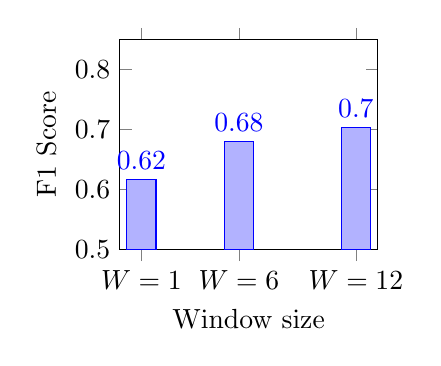
\begin{tikzpicture}
\begin{axis}[
    ybar,
    bar width=1.5,
    width=0.4\textwidth,
    height=0.35\textwidth,
    xlabel={Window size},
    ylabel={F1 Score},
    xtick={1, 6, 12},
    xticklabels={$W=1$, $W=6$, $W=12$},
    ymin=0.5, ymax=0.85,
    nodes near coords,
]
\addplot coordinates {(1, 0.6168) (6, 0.6804) (12, 0.7033)};
\end{axis}
\end{tikzpicture}
\caption{F1 score vs.\ window size.}
\label{fig:abl_window}
\end{figure}

\subsubsection{Temporal Columns}

The \texttt{sin\_hour} and \texttt{cos\_hour} features encode time-of-day. Table~\ref{tab:abl_temporal} and Figure~\ref{fig:abl_temporal} show that including them improves F1 from 0.686 to 0.703, indicating that the model benefits from explicit temporal conditioning.

\begin{table}[H]
\centering
\caption{Ablation: temporal columns.}
\label{tab:abl_temporal}
\small
\begin{tabular}{@{}lrrrr@{}}
\toprule
\textbf{Setting} & \textbf{Acc.} & \textbf{Prec.} & \textbf{Rec.} & \textbf{F1} \\ \midrule
Without temporal & 0.8258 & 0.9057 & 0.5518 & 0.6858 \\
With temporal    & 0.8323 & 0.9009 & 0.5767 & 0.7033 \\ \bottomrule
\end{tabular}
\end{table}

\begin{figure}[H]
\centering
\begin{tikzpicture}
\begin{axis}[
    ybar,
    bar width=0.6,
    width=0.4\textwidth,
    height=0.32\textwidth,
    symbolic x coords={Without, With},
    xtick=data,
    xticklabels={Without temporal, With temporal},
    x tick label style={font=\small},
    ymin=0.65, ymax=0.75,
    ylabel={F1 Score},
    nodes near coords,
]
\addplot coordinates {(Without, 0.6858) (With, 0.7033)};
\end{axis}
\end{tikzpicture}
\caption{F1 score: without vs.\ with temporal columns.}
\label{fig:abl_temporal}
\end{figure}

\subsubsection{Physics-Aware Mechanism}

We ablate how physics is integrated into the Physics-Aware ANN. \textbf{Loss-only}: the physics loss is added to the classification loss, but the leak head receives only the shared hidden representation (no predicted pressure/flow). \textbf{Moderate coupling} (current): the leak head additionally receives 5 features derived from predicted pressure and flow (mean, std, range), as described in the model architecture. Table~\ref{tab:abl_physics} and Figure~\ref{fig:abl_physics} show that moderate coupling improves F1 from 0.70 to 0.72 on a 100-scenario subset, indicating that feeding physics-derived features into classification helps beyond the regularizing effect of the loss alone.

\begin{table}[H]
\centering
\caption{Ablation: physics-aware mechanism (100 scenarios).}
\label{tab:abl_physics}
\small
\begin{tabular}{@{}llr@{}}
\toprule
\textbf{Variant} & \textbf{Description} & \textbf{F1} \\ \midrule
Loss only & Physics loss only; no pressure/flow in leak head & 0.70 \\
Moderate coupling & Predicted pressure/flow features in leak head & 0.72 \\ \bottomrule
\end{tabular}
\end{table}

\begin{figure}[H]
\centering
\begin{tikzpicture}
\begin{axis}[
    ybar,
    bar width=0.5,
    width=0.45\textwidth,
    height=0.32\textwidth,
    symbolic x coords={Loss only, Moderate coupling},
    xtick=data,
    x tick label style={font=\small},
    ymin=0.65, ymax=0.78,
    ylabel={F1 Score},
    nodes near coords,
]
\addplot coordinates {(Loss only, 0.70) (Moderate coupling, 0.72)};
\end{axis}
\end{tikzpicture}
\caption{Physics-aware mechanism: loss-only vs.\ moderate coupling.}
\label{fig:abl_physics}
\end{figure}

\bibliographystyle{IEEEtran}
\bibliography{References/S1944398624107059,
References/pmc_11647635,
References/citation-393247205,
References/Exported_Items-stgnn,
References/pinn_secure,
References/S0952197623002464,
References/citations-20251115T090154,
References/citations-probability,
References/we_emailed,
References/leakdb,
References/gnn_leak
}

\end{document}

